% !TEX TS-program = XeLaTeX
% Commands for running this example:
% 	 xelatex ICEE2009_farsi
% 	 bibtex8 -W -c cp1256fa ICEE2009_farsi
% 	 xelatex ICEE2009_farsi
% 	 xelatex ICEE2009_farsi
% End of Commands
\documentclass[11pt,a4paper,twocolumn]{article}
% Mahmood Amintoosi, http:/profsite.sttu.ac.ir/amintoosi
% m.amintoosi@gmail.com
% این فایل و فایلهای ضمیمه‌ی آن از سایت www.parsilatex.com قابل برداشت هستند.
% محمود امین طوسی - دانشگاه حکیم سبزواری
% این مقاله در هفدهمین کنفرانس مهندسی برق ایران در اردیبهشت ۸۸ ارائه شده است.

% شما می‌توانید از این فایل به عنوان یک الگو برای مقالات خود استفاده نمایید.

% برای پردازش پس از یکبار استفاده از xelatex با استفاده از دستور زیر لیست مراجع را تولید نمایید:
% bibtex ICEE2009_farsi
% و سپس دوبار استفاده از xelatex.

\usepackage{setspace}
\usepackage{subfigure}
\usepackage{algorithm}
\usepackage{algorithmic}
\usepackage{graphicx}
\usepackage{amsmath}
\usepackage[colorlinks, citecolor=blue]{hyperref}

\usepackage[top=25mm, bottom=25mm, left=20mm, right=20mm]{geometry}
\setlength{\columnwidth}{82mm}
\setlength{\columnsep}{6mm}

\usepackage{xepersian}
\settextfont[Scale=1]{XB Niloofar}
\setlatintextfont[Scale=.9]{Times New Roman}
\setdigitfont{XB Zar}

% استفاده از حالت خوابیده به چپ قلم ایکس‌بی‌زر مشابه با حالت ایرانیک در فارسی‌تک
\setiranicfont[Scale=.9]{XB Zar Oblique}
\defpersianfont\TitleBold[Scale=1]{XB Niloofar Bold}
\defpersianfont\AbstractBold[Scale=.92]{XB Niloofar Bold}

% تغییر فونت برچسب شکل‌ها، با استفاده از بسته زیر اندازه و نوع قلم برچسب شکل‌ها و جداول را در کل سند مشخص می‌کنیم. در حال حاضر (نسخه ۱.۰.۲ زی‌پرشین، این بسته با زی‌پرشین کاملاً سازگار نشده است. مسئولیت استفاده از آن با خودتان است ولی انشاءالله در نسخه‌ی بعدی زی‌پرشین این بسته هم سازگار شده و خواهید توانست آنرا قبل از بسته زی‌پرشین بکار گیرید.
% \usepackage[margin=0mm,font={small},labelfont={small,bf}]{caption}

% حذف عبارت چکیده
\renewcommand{\abstractname}{}

% اختصاص - به عنوان جداکننده شماره بخش و زیربخش
\SepMark{-}

% به صورت پیش‌فرض بعد از شماره بخش - نداریم، مگر آنکه شماره زیر بخش پس از آن آمده باشد. از آنجا که مطابق قالب کنفرانس در هر صورت
% پس از شماره بخش و شماره زیربخش به جداکننده نیاز داریم از دستورات زیر استفاده می‌کنیم:
\makeatletter
\renewcommand \thesection {\@arabic\c@section\@SepMark}
\renewcommand \thesubsection {\thesection\@arabic\c@subsection\@SepMark}
\makeatother

% تغییر نام algorithm به الگوریتم
\floatname{algorithm}{الگوریتم}

%\numberwithin{table}{section}
\onehalfspacing

\newcommand\femph[1]{\lr{''}#1\lr{``}}
\newcommand{\SR}{وضوحِ برتر }%{\textiranic{ وضوحِ برتر }}
\newcommand{\HR}{وضوح بالا }
\newcommand{\registration}{ثبت تصویر }
\newcommand{\fusion}{آمیختن }
\newcommand{\fused}{آمیخته }

\newcommand{\warp}{\mathbf{W}(\mathbf{x};\mathbf{p})}
\newcommand{\IWarp}{I(\mathbf{W}(\mathbf{x};\mathbf{p}))}
\newcommand{\round}[2]{\frac{\partial{#1}}{\partial{#2}}}
\newcommand{\roundB}[2]{\frac{\partial{\mathbf{#1}}}{\partial{\mathbf{#2}}}}

% با دستور زیر اندازه فرمولها را تغییر می‌دهیم. این دستور با فونت اندازه ۱۲ به خوبی کار می‌کند ولی با فونت اندازه ۱۱ که دراین مقاله استفاده نموده‌ام که ۶ صفحه بیشتر نشود، مشکلاتی دارد. به سایت: زیر مراجعه فرمایید: http://www.latex-community.org/forum/viewtopic.php?f=5&t=1792
\DeclareMathSizes{10.95}{9.2}{7.3}{5.5} %12,10,8,6

\thispagestyle{empty}

% برای اینکه چکیده حاشیه نداشته باشد
\renewcommand\abstract{}

%\expandafter\renewcommand\csname lr\endcsname[2][]{\LR{\resetlatinfont#2}}
%\newcommand{\latinindex}[1]{\index{\lr{#1}}}


\begin{document}
\title{
%\vspace{13mm} برای مطابقت با استیل کنفرانس این خط باید از حالت توضیح خارج شود.
\TitleBold{ثبت تصویر مبتنی بر شباهت ساختاری تصاویر با کاربرد در \SR}}
\author{محمود امین‌طوسی، محمود فتحی و ناصر مزینی\\
دانشگاه علم و صنعت ایران، دانشکده مهندسی کامپیوتر\\
\lr{\small\{mAmintoosi,mahFathy,Mozayani\}@iust.ac.ir}
}
% برخی دستورات زیر برای آن گذاشته شده‌اند که چکیده به صورت تک ستونی باشد
\twocolumn[
\begin{@twocolumnfalse}
\date{}
\maketitle

\begin{abstract}
\AbstractBold
{
\vspace{-5mm}
چکیده -
روش لوکاس-کاناد از جمله معروف‌ترین روش‌های ثبت تصویر مبتنی بر ناحیه است که گونه‌های مختلفی از آن تاکنون ارائه شده است. هدف اصلی در روشهای مختلف ثبت تصویر پیدا کردن پارامترهای مدل تبدیل، برای نگاشت دقیق یک تصویر بر روی مختصات تصویر دیگر است. در الگوریتم لوکاس-کاناد این امر از طریق کمینه‌سازی یک تابع مشخص کننده‌ی میزان تفاوت یک تصویر و تبدیل شده‌ی دیگری حاصل می‌شود. معمولاً تابع مذکور مربع تفاضلات بین دو تصویر در نظر گرفته می‌شود. در این مقاله از معیار شباهت ساختاری دو تصویر به عنوان ضریبی برای این تابع استفاده شده است. نحوه‌ی لحاظ کردن این معیار شباهت در فرمولبندی الگوریتم لوکاس-کاناد به صورت ریاضی بیان شده است. کمینه‌سازی مورد نظر با استفاده از شیوه‌ی بهینه‌سازی لونبرگ-مارکورت انجام شده است. نتایج پیاده‌سازی‌های انجام شده برتری شیوه‌ی پیشنهادی را در مقایسه با الگوریتم اصلی لوکاس-کاناد (با روشهای کمینه‌سازی گوس-نیوتن و لونبرگ-مارکورت) از نقطه نظر سرعت همگرائی نشان می‌دهد. همچنین کارائی شیوه‌ی پیشنهادی در مسئله‌ی وضوح برتر در مقایسه با چند روش دیگر نشان داده شده است.}
 \end{abstract}
{کلید واژه‌ها}- \fusion، ثبت تصویر، لونبرگ-مارکورت، موجک، وضوح برتر.\\
\end{@twocolumnfalse}]
% حذف شماره صفحات
\thispagestyle{empty}
\pagestyle{empty}

\section{مقدمه}
یکی از  مهمترین مسائل در حوزه‌ی پردازش تصویر و بینائی ماشین \textiranic{ ثبت تصویر} می‌باشد. هدف از \registration پیدا کردن تبدیل مناسب بین دو یا چند تصویر از یک صحنه است. در حالت کلی، باید تناظری یکتا بین یک نقطه از یک تصویر و نقطه‌ای دیگر از تصویر دوم  به نحوی پیدا نمود که هر دو نشان‌دهنده‌ی یک نقطه از صحنه باشند. 
 مسئله‌ی \registration قرابت نزدیکی با مسائل \textiranic{ تخمین حرکت}\LTRfootnote{ Motion Estimation}، \textiranic{ تصحیح حرکت}\LTRfootnote{ Motion Compensation} و \textiranic{ تطابق تصویر}\LTRfootnote{ Image Matching} دارد.

«ثبت تصویر» نقشی کلیدی در مسئله‌ی \textiranic{ وضوح برتر}\LTRfootnote{ Super-Resolution} دارد. هدف در  تکنیکهای \SR، عبارت است از ترکیب یک دنباله از تصاویر با وضوح پایین، نویزی و مات برای تولید یک تصویر یا یک دنباله از تصاویر با وضوح بالاتر. یک مرحله‌ی اصلی در این تکنیکها، تنظیم تصاویر ورودی بر روی یک شبکه‌ی مشترک و ترکیب مناسب آنهاست. معمولاً تنظیم تصاویر نسبت به یک تصویر مرجع صورت می‌پذیرد. وابستگی کیفیت تصویر نهایی به دقت مرحله‌ی ثبت تصویر امری واضح در مسئله‌ی وضوح برتر است \cite{Schultz96extraction}، فلذا هر پیشرفتی در این مرحله می‌تواند تاثیر بسزائی در نتیجه‌ی وضوح برتر داشته باشد. 
روشهای مواجهه با مسئله‌ی ثبت تصویر را می‌توان به دو دسته‌ی کلیِ \textiranic{ مبتنی بر ویژگی}
%\LTRfootnote{ Feature-based methods}
 و \textiranic{ مبتنی بر ناحیه}
%\LTRfootnote{ Area-based methods}
 تقسیم‌بندی نمود \cite{Zitova03image}. متدهای مبتنی بر ناحیه، در صورت مقداردهی اولیه‌ی مناسب می‌توانند به نتایجی با دقت بالا منتهی شوند. از جمله معروف‌ترین روشهای مبتنی بر ناحیه می‌توان به شیوه‌ی لوکاس-کاناد\LTRfootnote{ Lucas-Kanade}\cite{Lucas81iterative} اشاره نمود که در این مقاله از آن استفاده خواهد شد.
% که بنیان مقاله‌ی ایرانی و پِلگ\LTRfootnote{ Irani, Peleg}\cite{Irani91improving}، یکی از مهمترین مقالات در زمینه‌ی \SR می‌باشد. 

 اخیراً نویسندگان در \cite{Amintoosi08reconstruction,Amintoosi09regional} شیوه‌ای مشتمل بر استفاده از تصاویر آموزشی با وضوح بالا را برای افزایش وضوح تصویر ورودی ارائه نموده‌اند؛ در مقالات فوق‌الذکر مواردی مورد لحاظ قرار نگرفته است که در این مقاله به موارد زیر پرداخته خواهد شد:
 \begin{enumerate}
 \item در \cite{Amintoosi08reconstruction} برای ثبت تصویر فقط از یک شیوه‌ی مبتنی بر ویژگی استفاده شده است، در حالیکه این شیوه همیشه نتایج دقیقی تولید نمی‌کند؛ در این مقاله شیوه‌ی ثبت تصویر لوکاس-کاناد با استفاده از معیار شباهت ساختاری دو تصویر \cite{Wang04image} بهبود داده شده و در شیوه‌ی ارائه شده در \cite{Amintoosi08reconstruction} بکار گرفته شده است؛
 \item در \cite{Amintoosi08reconstruction,Amintoosi09regional} مرحله‌ی همرنگ نمودن\LTRfootnote{ Blending} تصاویر مورد ترکیب، بدون درز\LTRfootnote{ Seam-less} نبوده است؛ در این مقاله با استفاده از روش \textiranic{ همرنگ‌سازی چند بانده}
%\LTRfootnote{ Multi-band Blending}
\cite{Burt83multiresolution} این نقیصه برطرف شده است.
  \end{enumerate}

% چون پس از شماره بخشها - گذاشته‌ایم دستور زیر هم تحت تاثیر قرار گرفته است.  
% در بخش \ref{Sec:TheProposedMethod} شیوه‌ی پیشنهادی، در بخش \ref{Sec:ExperimentalResults} نتایج پیاده‌سازی‌ها و در انتها جمع‌بندی آورده شده است.
 در بخش ۲ شیوه‌ی پیشنهادی، در بخش ۳ نتایج پیاده‌سازی‌ها و در انتها جمع‌بندی آورده شده است.
%$SSIM$\LTRfootnote{ Structural SIMilarity (SSIM)}
%%%%%%%%%%%%%%%%%%%%%%%%%%%%%%% \section{شیوه‌ی پیشنهادی و نتایج}
\section{شیوه‌ی پیشنهادی}\label{Sec:TheProposedMethod}
 در شیوه‌ی پیشنهادی برای وضوح برتر توسط نگارندگان در \cite{Amintoosi08reconstruction}، هر یک از تصاویر باوضوح بالا، به عنوان تصویر آموزشی، متناظر با قسمتی از تصویرِ باوضوح پایین هستند.  تصاویر آموزشی می‌توانند تفاوتهایی با تصویر اصلی از نقطه نظر شدت روشنائی یا زاویه‌ی اخذ داشته باشند. 
 این تفاوتها می‌تواند ناشی از برداشت عکسها در زمانهای متفاوت و یا با دوربینهای متفاوت و از زوایای مختلف باشد. در این شیوه ابتدا تصویر با وضوح پایین به اندازه‌ی مطلوب بزرگ شده و سپس  تبدیل مناسبی برای نگاشت هر یک از تصاویر آموزشی بر روی تصویر مورد نظر با استفاده از  نقاط کلیدی \lr{SIFT}\LTRfootnote{ Scale Invariant Feature Transform (SIFT)} و الگوریتم \lr{RANSAC}\LTRfootnote{ RANdom SAmple Consensus (RANSAC)} در قالب ماتریس هوموگرافی
%\LTRfootnote{ Homography matrix}
 پیدا می‌شود. در انتها تصویرِِ باوضوح بالای نگاشت شده، با تصویر باوضوح پایین ورودی
% \fused\LTRfootnote{ Fused}
ترکیب می‌شود.
 چارچوب کلی کار در این مقاله در شکل~\ref{fig:OneLR_oneHR} آمده است. دو مرحله‌ی « دقیق‌تر نمودن مدل با استفاده از ثبت تصویر مبتنی بر ناحیه» و «همرنگ نمودن تصاویر در نواحی مرزی» در این مقاله اضافه شده‌اند. از آنجا که ذکر روش کار برای یک یا چند تصویر آموزشی تفاوتی ندارد، در اینجا فرض بر آن است که فقط از یک تصویر آموزشی استفاده می‌شود.

%------------------------- Visio Chart, OneLR_OneHR
\begin{figure}[t]
%\centerline{\XeTeXpdffile "Images/OneLR_oneHR.pdf" height 14cm}
\centering 
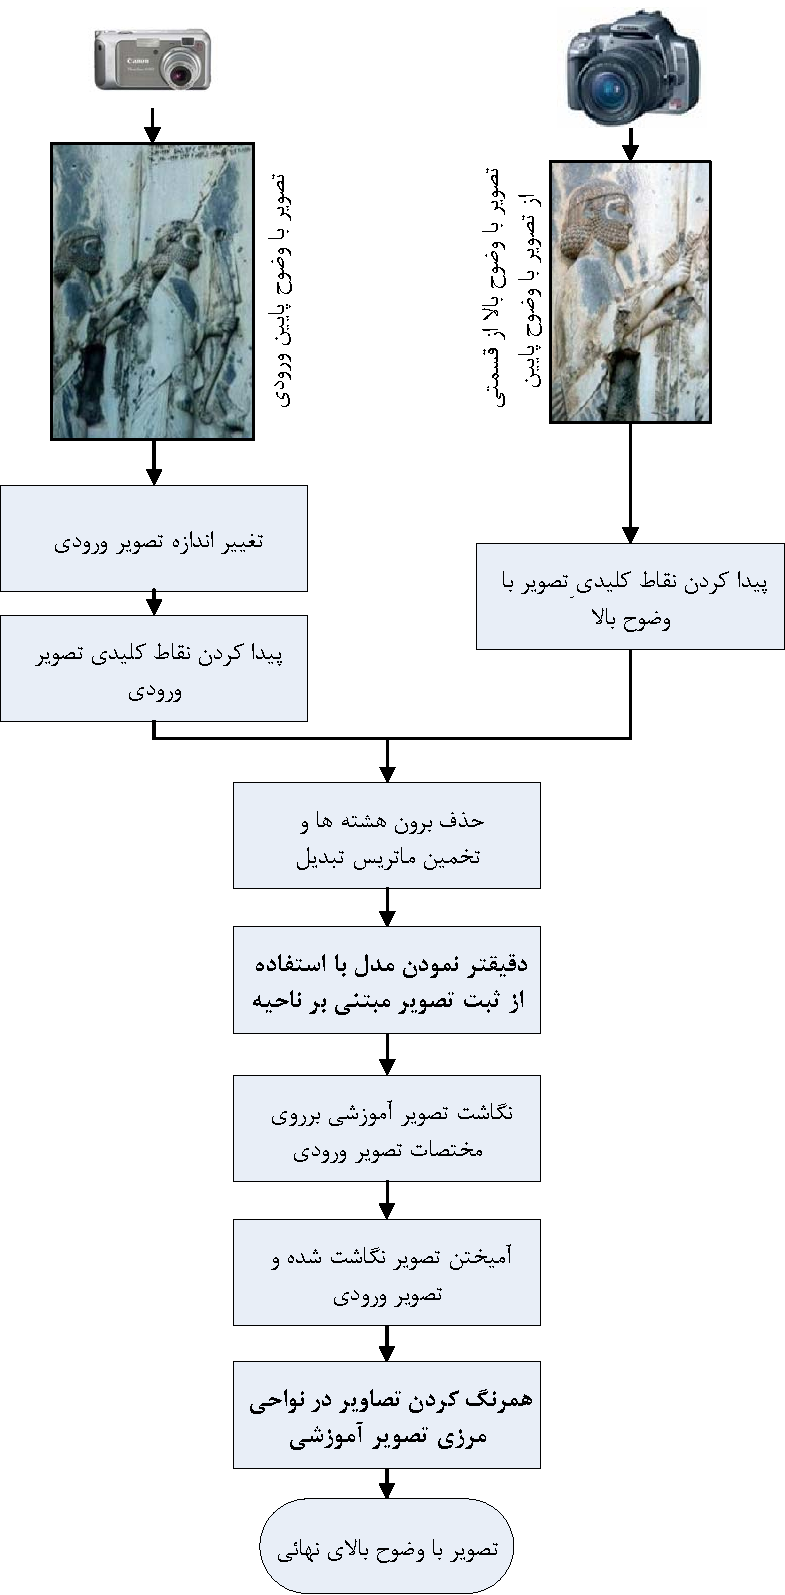
\includegraphics[width=70mm]{Images/OneLR_oneHR.pdf}
\caption{چارچوب کلی شیوه‌ی پیشنهادی.}\label{fig:OneLR_oneHR}
\end{figure}


مهمترین قسمت در کار حاضر استفاده از معیار مقایسه‌ی ساختاری دو تصویر ($SSIM$) برای بهبود شیوه‌ی ثبت تصویر لوکاس-کاناد\cite{Lucas81iterative} می‌باشد. در مراجع از فرمولبندی‌های متفاوتی برای بیان این شیوه استفاده شده است. در این مقاله از فرمولبندی ذکر شده در \cite{Baker04lucas-kanade20part1} استفاده خواهیم نمود و لذا مروری بر این فرمولبندی ضروری می‌باشد که در ادامه ذکر خواهد شد. پس از آن نگاهی بر معیار مقایسه‌ی $SSIM$ داشته و سپس روش پیشنهادی بر اساس آنها بیان خواهد شد.

\subsection{الگوریتم لوکاس-کاناد}
 هدف در شیوه‌ی ثبت تصویر لوکاس-کاناد\cite{Lucas81iterative} کمینه‌سازی مجموع مربع تفاضلات زیر بین تصویر آموزشیِ $T(\mathbf{x})$ و نگاشت تصویر ورودیِ $I(\mathbf{x})$ است:
 \begin{equation}\label{eq:SSD_L2Norm}
    SSD=\sum_x[\IWarp-T(\mathbf{x})]^2
\end{equation}
که در آن $\warp$ بیانگر مدل تبدیل‌ (در اینجا پروجکتیو)، $\mathbf{p}=(p_1,\dots,p_8)^T$ پارامترهای مدل تبدیل، $\IWarp$ نگاشت تصویر ورودی $I$ بر روی مختصات تصویر آموزشی $T$ و $\mathbf{x} =(x,y)^T$ مختصات یک پیکسل می‌باشد.
 کمینه‌سازی \eqref{eq:SSD_L2Norm} نسبت به $\mathbf{p}$ انجام می‌شود. 
در شیوه‌ی لوکاس-کاناد فرض بر آن است که در ابتدا تخمینی از مدل دردست بوده و در یک فرآیند تکراری این تخمین بهبود داده می‌شود؛
در هر دور ابتدا عبارت زیر بر اساس $\triangle\mathbf{p}$ کمینه شده:
\begin{equation}\label{eq:SSD_L2Norm_deltap}
    \sum_x[I(\mathbf{W}(\mathbf{x;\mathbf{p+\triangle p}}))-T(\mathbf{x})]^2
\end{equation}
 و سپس پارامترها بروزرسانی می‌شوند:
\begin{equation}
    \mathbf{p}\leftarrow\mathbf{p+\triangle p}
\end{equation}
دو مرحله‌ی فوق تا مادامیکه الگوریتم همگرا نشده است تکرار خواهند شد. در فرآیند کمینه‌سازی، $\mathbf{\triangle p}$ به صورت زیر محاسبه می‌شود:
\begin{equation}\label{eq:deltap}
    \triangle\mathbf{p} = H^{-1} \sum_x[\nabla I\roundB{W}{p}]^T[T(\mathbf{x})-\IWarp]
\end{equation}
که در آن $H$، ماتریس هسین تقریبی\LTRfootnote{ Approximate Hessian Matrix}، به صورت زیر بدست می‌آید:
\begin{equation}\label{eq:Hessian}
    H = \sum_x[\nabla I\roundB{W}{p}]^T[\nabla I\roundB{W}{p}]
\end{equation}
این مراحل در الگوریتم \ref{alg1} نشان داده شده است \cite{Baker04lucas-kanade20part1}.
گونه‌های مختلفی از این الگوریتم پیشنهاد شده‌اند. سلزکی\LTRfootnote{ Szeliski} در \cite{Szeliski96video} از روش بهینه‌سازی لونبرگ-مارکورت برای قسمت بهینه سازی آن استفاده نموده است که اساس کار ما در بخش‌های آتی می‌باشد.
\begin{algorithm}[t]
\caption{الگوریتم ثبت تصویر لوکاس-کاناد مبتنی بر بهینه‌سازی گوس-نیوتون \lr{(LK-GN)}.} \label{alg1}
\singlespacing
\begin{latin}
\textbf{Input}:
The reference image $I$ and template image $T$.\\
\textbf{Output}: Reg. parameters
$\mathbf{p}=(p_1,\dots,p_n)^T$ as the warp model $\warp$.
\begin{algorithmic}[1]
\REPEAT
  \STATE Warp $I$ with $\warp$ to compute $\IWarp$. 
  \STATE Compute the error image $T(x)-\IWarp$ 
  \STATE Warp the gradient $\nabla I$ with $\warp$. \STATE Evaluate the Jacobian
    $\roundB{W}{p}$ at $(\mathbf{x;p})$. 
  \STATE Compute the steepest descent images $\nabla I\roundB{W}{p}$. 
  \STATE \label{line:Hessian} Compute the Hessian matrix using Equation
    \eqref{eq:Hessian}. 
  \STATE Compute $[\nabla I\roundB{W}{p}]^T$ and $[T(x)-\IWarp]$ 
  \STATE \label{alg1:deltap} Compute $\triangle\mathbf{p}$ using Equation \eqref{eq:deltap} 
  \STATE Update the parameters $\mathbf{p}\leftarrow\mathbf{p}+\triangle\mathbf{p}$ 
\UNTIL{$||\triangle\mathbf{p}||\leq\epsilon$ or Reaching to Maximum Iteration allowed}
\end{algorithmic}
\end{latin}
\end{algorithm}


\subsection{ارزیابی خطا با محک $SSIM$}
در \cite{Wang04image} محک $MSSIM$\LTRfootnote{ Mean Structural SIMilarity} برای اندازه‌گیری کیفیت یک تصویر، به صورت زیر تعریف شده است:
\begin{equation}\label{eq:MSSIM}
    MSSIM(X,Y) = \frac{1}{M}\sum_{j=1}^M SSIM(x_j,y_j)
\end{equation}
که در آن $X$ تصویر مرجع، $Y$ تصویر تخریب شده؛ $x_j$ و $y_j$ اجزاء $j$امین پنجره در تصاویر و $M$، تعداد پنجره‌ها می‌باشد. 
$SSIM(x,y)$ مطابق زیر تعریف می‌شود:
\begin{equation}\label{eq:SSIM}
    SSIM(x,y)=\frac{(2\mu_x\mu_y+C_1)(2\sigma_{xy}+C_2)}{(\mu_x^2+\mu_y^2+C_1)(\sigma_x^2+\sigma_y^2+C_2)}
\end{equation}
که در آن $C_1,C_2$ ثوابتی برای پایداری و \lr{$\mu_x, \sigma_x$, $\sigma_{xy}$} تخمین آمارگان محلی تصویر هستند که در \cite{Wang04image} تعریف شده‌اند. 


\subsection{لحاظ کردن $SSIM$ در الگوریتم لوکاس-کاناد}
$MSSIM(X,Y)$ به نحوی تعریف شده است که هر چه دو تصویر به هم شبیه‌تر باشند این معیار به 1 نزدیک‌تر خواهد بود. اما ما در اینجا به معیاری نیاز داریم که میزان تفاوت دو تصویر را نشان دهد. به این منظور از $-SSIM$ استفاده نموده و آنرا $SDIS$\LTRfootnote{ Structural DISsimilarity} می‌نامیم:
\begin{equation}\label{eq:SDISneg}
    SDIS(x,y) = -SSIM(x,y)
\end{equation}
بر اساس این تعریف، تفاوت بیشتر دو تصویر مقدار بزرگتری از $SDIS$ را نتیجه خواهد داد.
$SSIM$ بین پیکسلهای متناظر دو تصویر تعریف می‌شود؛ تصویری که از مقایسه‌ی شباهت تک‌ تک پیکسلهای دو تصویر با این معیار حاصل می‌شود در \cite{Wang04image}، \lr{$SSIM\ map\ image$} نامیده شده است، به صورت متناظر در اینجا تصویری را که از مقایسه‌ی تفاوت دو تصویر بر اساس \eqref{eq:SDISneg} ایجاد می‌شود \lr{$SDIS\ map\ image$} می‌نامیم. از آنجا که در ادامه از این معیار به عنوان میزان خطا در ثبت تصویر استفاده خواهیم کرد آنرا با $E_{SDIS}$ نشان می‌دهیم.  با درنظر گرفتن این معیار به عنوان ضریبی از میانگین مربعات خطا، رابطه‌ی \eqref{eq:SSD_L2Norm} به صورت زیر در خواهد آمد:
\begin{equation}\label{eq:SSD_L2Norm_SDIS}
    \sum_x E_{SDIS}.[\IWarp-T(\mathbf{x})]^2
\end{equation}
که در آن منظور از نقطه، ضرب عناصر نظیر در دو ماتریس است. برای کمینه‌سازی \eqref{eq:SSD_L2Norm_SDIS}، با یک شیوه‌ی تکراری مشابه \eqref{eq:SSD_L2Norm_deltap} بایستی تابع زیر را کمینه نماییم:
\begin{equation}\label{eq:SSD_SDIS_deltap}
    \sum_x E_{SDIS}.[I(\mathbf{W}(\mathbf{x;\mathbf{p+\triangle p}}))-T(\mathbf{x})]^2
\end{equation}
که در آن $E_{SDIS}$ در $\warp$ ارزیابی می‌شود. با انجام بسط تیلور مرتبه‌ی اول روی $I(\mathbf{W}(\mathbf{x;\mathbf{p+\triangle p}}))$ داریم:
\begin{align}
    &SSD =\label{eq:SSD_SDIS_Taylor} \\
	&\sum_x E_{SDIS}.[\IWarp+\nabla I\roundB{W}{p}\triangle \mathbf{p}-T(\mathbf{x})]^2 \nonumber
\end{align}
که در آن:
$\nabla I=(\round{I}{x},\round{I}{y})$ گرادیان تصویر $I$، ارزیابی شده در $\warp$ و $\roundB{W}{p}$ ژاکوبین مدل تبدیل می‌باشد.

از ادامه مطلب صرفنظر می‌کنیم.
\begin{figure}[tp]
\centering \subfigure[{تصویر با وضوح پایین ورودی}]{\label{fig:Results:LR}
\includegraphics*[width = .25\columnwidth]{Images/Kamandar_LR_Nearest.jpg}}%\vspace{2mm}
\subfigure[{تصویر آموزشی با وضوح بالا}]{\label{fig:Results:HR}
\includegraphics*[width = .25\columnwidth]{Images/Neyzeh_dar.jpg}}%\hspace{2mm}
\subfigure[{نتیجه نهایی در \lr{SNR=90dB}}]{\label{fig:Results:Final}
\includegraphics*[width = .5\columnwidth]{Images/Kamandar_blendXFus_FA-LM-SSIM.jpg}}
 \caption{نتیجه نهایی افزایش وضوح تصویر ورودی(ا) با استفاده از تصویر (ب) و با روش پیشنهادی در شکل \ref{fig:OneLR_oneHR} که دقیق‌تر نمودن ثبت تصویر در آن با الگوریتم2 و همرنگ نمودن بدون درز با شیوه‌ی ارائه شده در \cite{Burt83multiresolution} انجام شده است.}
\label{fig:Results}
\end{figure}

\section{نتایج پیاده‌سازی}\label{Sec:ExperimentalResults}
شیوه‌ی پیشنهادی  با شیوه‌ی اصلی لوکاس-کاناد\cite{Lucas81iterative} در الگوریتم1 (\lr{LK-GN}) و شیوه‌ی لوکاس-کاناد با روش بهینه‌سازی لونبرگ-مارکورت\cite{Szeliski96video} (\lr{LK-LM})، از نظر میانگین تعداد تکرار تا همگرائی و میانگین خطا (\LTRfootnote{ Root Mean Square}\lr{RMS}) و در مقادیر مختلف نویز مقایسه شده است. تصاویر مورد استفاده در شکل‌های \ref{fig:Results:LR} و \ref{fig:Results:HR} نشان داده شده‌اند. این تصاویر از یکی از سی‌دی‌های مربوط به نقش برجسته‌ی داریوش در بیستون اخذ شده‌اند. همانگونه که در شکل \ref{fig:Results} مشاهده می‌شود دو تصویر از نظر وضوح، شدت روشنایی و رنگ‌بندی با یکدیگر متفاوت هستند. تفاوت زاویه‌ی اخذ دو تصویر نیز در هنگام نگاشت پروجکتیو تصویر \ref{fig:Results:HR} بر روی تصویر \ref{fig:Results:LR} -که در اینجا نشان داده نشده است- مشخص می‌باشد.

 هدف اصلی بالابردن وضوح قسمت متناظر با تصویر \ref{fig:Results:HR} در تصویر \ref{fig:Results:LR} با شیوه‌ی نشان داده شده در شکل \ref{fig:OneLR_oneHR} است. در مقایسات انجام شده، تمام مراحل شکل \ref{fig:OneLR_oneHR} به استثنای مرحله‌ی «دقیق‌تر نمودن مدل با استفاده از ثبت تصویر مبتنی بر ناحیه» یکسان بوده است. نقطه‌ی آغازین بهینه‌سازی در هر سه الگوریتم، تخمین ماتریس تبدیل بدست آمده در مرحله‌ی قبل با استفاده از الگوریتم \lr{RANSAC} می‌باشد. 
%\newpage
ماهیت تصادفی الگوریتم \lr{RANSAC} موجب می‌شود که در هر اجرا تخمینی متفاوت با اجرای دیگر داشته باشیم. لذا هر 
%اجرای الگوریتم شکل \ref{fig:OneLR_oneHR} 
آزمایش را می‌توان جدا از دیگری دانست. 


\subsection{نتایج مقایسه‌ای ثبت تصویر}
هر سه شیوه‌ی فوق‌الذکر برای تصاویر شکل\ref{fig:Results} و در نرخ سیگنال به نویز\LTRfootnote{ Signal to Noise Ratio (SNR)} برابر با 70،50،30،10 و 90 \lr{dB} از تصویر با وضوح پایین اجرا شده‌اند. هر الگوریتم در هر \lr{SNR} 20 مرتبه اجرا شده است. 

شکل \ref{fig:Conv_Iter} میانگین تعداد تکرارها تا همگرا شدن را برای هر سه روش فوق و در مقادیر مختلف نویز نشان می‌دهد. در هیچ یک از آزمایشات روی این تصاویر، روش \lr{LK} واگرا نشده بود.

\begin{figure}[tp]
\centering
\includegraphics*[height=50mm, width = 0.7\columnwidth]{Images/Afsaran_mean_conv_iter.eps}
\caption{ میانگین تعداد تکرار مورد نیاز تا همگرائی.}
\label{fig:Conv_Iter}
\end{figure}

\subsection{کاربرد در وضوح برتر}
کیفیت بصری تصویر نهائی تولید شده، لازمه‌ی اعتبارسنجی هر الگوریتم \SR است. 
شکل \ref{fig:Results:Final} نتیجه‌ی نهائی افزایش وضوح تصویر \ref{fig:Results:LR} با استفاده از تصویر آموزشی \ref{fig:Results:HR} را
 نشان می‌دهد. ضریب بزرگ‌نمایی، 2 در نظر گرفته شده است. 
برای مقایسه‌ چند شیوه‌ی دیگر پیاده‌سازی شده‌اند. مقایسه‌ی تصاویر شکل \ref{fig:Katibeh} کیفیت برتر شیوه‌ی پیشنهادی را به خوبی نشان می‌دهد. به عنوان روش \fusion در روش پیشنهادی در این مقاله و روش ارائه شده در \cite{Amintoosi08reconstruction} از تبدیل موجک دوبیشز%\LTRfootnote{ Daubechies}
 و با 3 سطح استفاده شده است. روش مبتنی بر مثال ارائه شده در \cite{Freeman02example} نیز به منظور مقایسه پیاده‌سازی شده و برای حفظ سازگاری بلوکهای مجاور از شیوه‌ی پویش سطر به سطر ذکر شده در همان مرجع استفاده شده است. روشهای افزایش اندازه‌ی تصویرِ \lr{Replication} و \lr{Bicubic} در واقع جزو روشهای افزایش وضوح به حساب نمی‌آیند و نتایج آنها صرفاً برای مقایسه آمده است. ناپدید شدن درز در نواحی مرزی و دقیق‌تر بودن نگاشت در شیوه‌ی پیشنهادی مشخص است.

\begin{figure}[t!]
\centering 
\subfigure[روش بزرگنمائی \lr{Replication}]{ \label{fig:Katibeh:Nearest}
\includegraphics[width=35mm]{Images/Kamandar_LR_Nearest_Cropped.jpg}}
\hspace{2mm}
\subfigure[روش بزرگنمائی \lr{Bicubic}]{ \label{fig:Katibeh:Bicubic}
\includegraphics[width=35mm]{Images/Kamandar_LR_Cropped.jpg}}
\hspace{2mm}
\subfigure[روش  ارائه شده در \cite{Freeman02example}]{ \label{fig:Katibeh:Freeman}
\includegraphics[width=35mm]{Images/Kamandar_Freeman_Cropped.jpg}}
\hspace{2mm}
\subfigure[روش  ارائه شده در \cite{Amintoosi08reconstruction}]{ \label{fig:Katibeh:Fustruction}
\lr{\includegraphics[width=35mm]{Images/Kamandar_Fustruction_Cropped.jpg}}}
\hspace{2mm}
\subfigure[روش  پیشنهادی در این مقاله بدون مرحله‌ی آمیختن با تبدیل موجک]{\label{fig:Katibeh:AreaBasedXFus}
\includegraphics[width=35mm]{Images/Kamandar_blend_FA-LM-SSIM_Cropped.jpg}}
\hspace{2mm}
\subfigure[روش  پیشنهادی در این مقاله]{\label{fig:Katibeh:AreaBasedXFus}
\includegraphics[width=35mm]{Images/Kamandar_blendXFus_Fa-LM-SSIM_Cropped.jpg}}

\caption{بزرگ شده‌ی قسمتی از نتیجه‌ی اجرای شیوه‌های مختلف برای افزایش وضوح شکل \ref{fig:Results:LR}. دقیق‌تر بودن مدل در شیوه‌ی پیشنهادی نسبت به شیوه‌ی ذکر شده در \cite{Amintoosi08reconstruction} که فاقد ثبت تصویر مبتنی بر ناحیه است از مقایسه‌ی قسمت بالای نیزه در شکلهای (و) و (د) مشخص است.}
\label{fig:Katibeh} %% label for entire figure
\end{figure}


\section{جمع‌بندی}\label{Sec:Conclusion}
نویسندگان در \cite{Amintoosi08reconstruction} شیوه‌ای جدید برای افزایش وضوح یک تصویر با استفاده از یک تصویر آموزشی ارائه نموده بودند که در مقاله‌ی حاضر به رفع مشکلاتی از آن پرداخته شد. استفاده از یک روش ثبت تصویر مبتنی بر ناحیه به منظور دقیق‌تر شدن مدل نگاشت تصاویر و حذف مرزهای تصاویر با یک روش همرنگ‌سازی بدون درز مراحلی هستند که در کار قبلی انجام نشده بودند. نوآوری اصلی این مقاله لحاظ کردن معیار شباهت ساختاری دو تصویر در فرمولبندی شیوه‌ی معروف ثبت تصویر لوکاس-کاناد و استفاده از آن در وضوح برتر می‌باشد. نتایج پیاده‌سازی‌های انجام شده برتری شیوه‌ی ثبت تصویر پیشنهادی و همچنین کارائی آنرا در مسئله‌ی وضوح برتر در مقایسه با برخی از دیگر روشها نشان داده است.

\subsection*{سپاس‌گزاری}
مؤلفین وظیفه‌ی خود می‌دانند که از آقای دکتر \lr{Peter Kovesi} بابت توابع سودمند \lr{MATLAB} 
\LTRfootnote{ School of Computer Science \& Software Engineering, The University of
Western Australia:\hfill http://www.csse.uwa.edu.au/}
و آقایان وفا خلیقی، مصطفی واحدی و دکتر مهدی امیدعلی بابت زحمات و راهنمایی‌های ارزنده‌ی آنها در زمینه‌ی زی‌پرشین
\RTLfootnote{زی‌پرشین با لوگوی \lr{\XePersian} بسته‌ی حروف‌چینی رایگان فارسی مبتنی بر \lr{\LaTeXe} و تحت سیستم‌عامل‌های ویندوز، لینوکس و مک
 می‌باشد:\\
 {\lr{http://www.parsilatex.com/\hfill}}} (که این مقاله با آن آماده شده است) تشکر به عمل آورند. 



%\begin{latin}
{
% سه دستور زیر باعث می‌شوند که مراجع با قلم کوچکتر و با فاصله خطوط کمتر و با فاصله بین مراجع کم ظاهر شوند. 
% این حالت برای کاهش تعداد صفحات مقاله مناسب است.
% می‌توانید هر یک از آنها را comment نموده و خروجی را ملاحظه فرمایید.
\small
\singlespacing
\setlength{\itemsep}{-2ex}
%اگر از فایلهای سبک انگلیسی مانند latex8.bst یا ieeetr-fa استفاده کنید بایستی کل قسمت مراجع را در داخل یک محیط latin قرار دهید (که در حال حاضر comment شده است و دستور زیر را نیز از حالت comment خارج کنید.
%\renewcommand{\refname}{\rl{{مراجع}\hfill}}
\bibliographystyle{ieeetr-fa}%{latex8}%{IEEEtrans}
\bibliography{SR_References}
}
%\end{latin}

\end{document}